% =============================================================================
% Projeto GPTI -- Entrega P2B (PT-BR)
% Formatação: ABNT (classe abnTeX2, modo article), A4, Latin Modern, 12 pt,
% margens 3/2/3/2 cm, espaçamento 1,5, recuo de parágrafo 1,25 cm.
% Figura esperada em: out/Figura_1_Percurso_Dado_Pessoal.pdf
% (compilada a partir de figuras/Figura_1_Percurso_Dado_Pessoal.tex)
% =============================================================================
\documentclass[12pt,a4paper,article,oneside,english,brazil]{abntex2}

\usepackage[T1]{fontenc}
\usepackage[utf8]{inputenc}
\usepackage{lmodern}           % Latin Modern (fonte padrão do LaTeX, com T1)
\usepackage{amsmath}
\usepackage{graphicx}
\usepackage{array}
\usepackage{tabularx}
\usepackage[expansion=false]{microtype}

% Margens ABNT: superior 3 cm, inferior 2 cm, esquerda 3 cm, direita 2 cm
\setlrmarginsandblock{3cm}{2cm}{*}
\setulmarginsandblock{3cm}{2cm}{*}
\checkandfixthelayout

\setlength{\parindent}{1.25cm}
\setlength{\parskip}{0pt}
\setlength{\emergencystretch}{2em}

% Tabelas: sem filetes verticais (padrão IBGE adotado pela ABNT)
\newcolumntype{Y}{>{\raggedright\arraybackslash}X}
\renewcommand{\arraystretch}{1.2}

% Fonte/nota abaixo de tabelas e figuras (ABNT NBR 14724)
\newcommand{\fontetab}[1]{\par\vspace{3pt}{\small\noindent Fonte: #1\par}}

% Configuração DSQ(t_k)
\newcommand{\dsq}[1]{DSQ($t_{#1}$)}

\begin{document}

% ------------------------------- CAPA ----------------------------------------
\thispagestyle{empty}
\noindent\begin{minipage}[t][0.92\textheight]{\textwidth}
\centering
\SingleSpacing
\textbf{UNIVERSIDADE DE BRASÍLIA -- UNB\\
PROGRAMA DE PÓS-GRADUAÇÃO EM COMPUTAÇÃO APLICADA -- PPCA\\
DISCIPLINA: GESTÃO DE PROJETOS DE TI (GPTI)\\
PROFESSOR: Dr. JOÃO MELLO DA SILVA}

\vspace{1cm}

\textbf{Grupo Mobilizador Digital 1}: Gabriel Porto Oliveira, Marcus Vinícius Oliveira Reis, Suzy Alves Arcanjo e William de Almeida Silva.

\vspace{0.4cm}

\textbf{Grupo Reciclagem 1:} Filipe Alves de Sousa, Emanuel Brandão de Galvão Correia, Ruben Isaac Dias da Silva e Carlos Eduardo da Silva Papa.

\vspace{0.4cm}

\textbf{Grupo Aterro:} Lucien Rocha, Edvan Silva, Helton Garcia e Lucas Ferreira.

\vspace{3cm}

\textbf{PRIVACIDADE EM GÊMEOS DIGITAIS DO SISTEMA DE RESÍDUOS SÓLIDOS: CONSOLIDAÇÃO FSPC DE TRÊS SEGMENTOS}

\vfill

BRASÍLIA -- DF\\
2026
\end{minipage}
\clearpage

% ------------------------------ RESUMOS --------------------------------------
\begin{resumo}
Este artigo consolida três trabalhos da disciplina GPTI que descrevem gêmeos digitais de segmentos sucessivos do Sistema de Resíduos Sólidos (SRS) do Distrito Federal: o Mobilizador Digital (DM), que atua na origem junto ao cidadão; a Reciclagem via cooperativas de catadores (R3), que opera no galpão; e o Aterro sanitário (D), que recebe o rejeito na destinação final. Os três trabalhos usam a mesma lente sistêmica, Função, Estrutura, Processo e Contexto (FSPC), e partilham o paradigma do gêmeo digital como referência de decisão, e não como réplica do estado atual. A consolidação organizou o conteúdo dos três trabalhos em uma matriz FSPC $\times$ segmento e leu cada célula pelo domínio Privacidade do modelo SIPA (Sustentabilidade, Inovação, Privacidade e Análise de negócios com decisões ajustadas a riscos). Os resultados mostram que o mesmo dado pessoal atravessa os três gêmeos: nasce no DM como cadastro, perfil e geolocalização de domicílios, volta ao R3 como qualidade da separação por rota e chega ao aterro como suporte físico com dados residuais. Na Função, só o segmento do aterro trata a eliminação comprovada do dado como finalidade, e essa é a lacuna mais clara da literatura. Na Estrutura, as seis famílias de capacidades do Digital Twin Consortium são comuns aos três gêmeos, mas apenas o R3 atribui salvaguardas de privacidade a cada agente de inteligência artificial. No Processo, o R3 condiciona a evolução do gêmeo ao relatório de impacto à proteção de dados pessoais (RIPD), e o aterro mapeia ameaças LINDDUN por etapa do ciclo. No Contexto, PNRS e LGPD são comuns, mas a literatura raramente liga privacidade a direitos e instituições. O artigo propõe ler a cadeia como um sistema único de gêmeos interligados e declara o uso de inteligência artificial na consolidação.

\vspace{\onelineskip}
\noindent\textbf{Palavras-chave:} gêmeo digital; resíduos sólidos; privacidade; FSPC; SIPA; LGPD; gestão de projetos.
\end{resumo}

\begin{resumo}[Abstract]
\begin{otherlanguage*}{english}
This paper consolidates three course projects that describe digital twins of successive segments of the Federal District solid waste system: the Digital Mobilizer (DM), at the source; recycling through waste-picker cooperatives (R3), at the sorting facility; and the sanitary landfill (D), at final disposal. All three use the Function, Structure, Process and Context (FSPC) lens and treat the digital twin as a decision reference rather than a replica. We arranged their content in an FSPC $\times$ segment matrix and read each cell through the Privacy domain of the SIPA model. The same personal data travels across the three twins: it is created at the DM, returns to R3 as route-level sorting quality and reaches the landfill as physical media with residual data. Only the landfill segment treats verified data elimination as a function; only R3 assigns privacy safeguards to each AI agent; R3 gates twin evolution on a data protection impact assessment; and the landfill maps LINDDUN threats by stage. We also disclose how artificial intelligence was used in the consolidation.

\vspace{\onelineskip}
\noindent\textbf{Keywords:} digital twin; solid waste; privacy; FSPC; SIPA; LGPD; project management.
\end{otherlanguage*}
\end{resumo}

\newpage

% ------------------------------ 1 INTRODUÇÃO ---------------------------------
\section{INTRODUÇÃO}

O Sistema de Resíduos Sólidos (SRS) do Distrito Federal passou por uma reorganização profunda com o fechamento do Lixão da Estrutural, em janeiro de 2018. Durante décadas, o lixão recebeu a maior parte dos resíduos do DF e foi local de trabalho de centenas de catadores. Seu fechamento exigiu alternativas de destinação e de inclusão produtiva, em grande parte organizadas em cooperativas. No material da disciplina GPTI, o SRS é decomposto em componentes que correspondem às etapas do ciclo dos resíduos: Prevenção e Redução, Mobilizador Digital, Reuso, Reciclagem e Descarte. O sufixo CC, presente nas siglas dos componentes, indica que a operação ocorre via cooperativas de catadores, o que une educação ambiental, geração de renda e inclusão social.

Cada componente foi descrito por um grupo da disciplina na forma de dois gêmeos: um gêmeo real, que pertence ao mundo físico, e um gêmeo digital, que pertence ao mundo digital e pode usar toda a inteligência organizacional disponível nesse espaço. Três desses trabalhos cobrem segmentos sucessivos da mesma cadeia. O primeiro descreve o Mobilizador Digital 1 (DSRSDM-CC), que engaja a população na separação na origem. O segundo descreve o gêmeo digital da Reciclagem em cooperativas (DSRSR3-CC), que acompanha coleta seletiva, triagem, transformação e comercialização. O terceiro revisa a literatura sobre aterros sanitários sob a ótica FSPC e acrescenta o domínio Privacidade, propondo um gêmeo digital de projeto com uma camada de privacidade desde a concepção.

Os três trabalhos foram feitos em paralelo, por grupos diferentes, com buscas e artigos de referência próprios. Eles compartilham, porém, a mesma lente de descrição, Função, Estrutura, Processo e Contexto (FSPC), e o mesmo paradigma: o gêmeo digital deixa de ser réplica do estado atual e passa a ser referência para decidir como o sistema real deve evoluir. Essa base comum permite lê-los juntos. Uma leitura conjunta interessa porque os segmentos não são independentes. O trabalho do Mobilizador lembra que, se a população não separa corretamente os resíduos em casa, o Reuso, a Reciclagem e as cooperativas recebem material em menor quantidade e de pior qualidade, e uma parcela maior vai para o aterro. O trabalho da Reciclagem propõe devolver a qualidade da separação observada por rota ao Mobilizador. O trabalho do Aterro mostra que o resíduo carrega dados pessoais no próprio material, nos sistemas que o acompanham e nas pessoas que vivem dele.

A privacidade é o fio que mais se beneficia dessa leitura. A Lei Geral de Proteção de Dados Pessoais (LGPD, Lei 13.709/2018) trata a eliminação de dados como operação de tratamento (art. 5º, X). Descartar um suporte com dados pessoais é, portanto, tratar dados, e o aterro é o último elo dessa cadeia. Ao mesmo tempo, cada gêmeo digital acrescenta uma nova camada de coleta e cruzamento de dados, que pode proteger ou expor. Um dado coletado no aplicativo do Mobilizador pode ser cruzado no gêmeo da Reciclagem e reaparecer, como suporte físico, no aterro.

\subsection{Objetivo e perguntas}

Consolidar os três trabalhos em uma descrição única, organizada pelas quatro dimensões FSPC, destacando em cada dimensão os pontos relevantes de cada segmento e o que eles implicam para a privacidade. A consolidação se limita ao conteúdo dos três trabalhos base e às fontes que eles citam. Três perguntas orientam o texto:

\begin{list}{}{\setlength{\leftmargin}{0.635cm}\setlength{\itemsep}{0pt}\setlength{\topsep}{0pt}}
\item \textbf{P1.} O que cada segmento contribui, em cada dimensão FSPC, para a descrição do gêmeo digital do SRS?
\item \textbf{P2.} Onde os segmentos convergem e onde divergem no tratamento da privacidade?
\item \textbf{P3.} O que a leitura conjunta revela que nenhum trabalho isolado mostra?
\end{list}

O artigo segue esta ordem: referencial teórico (seção 2), método de consolidação (3), o sistema em questão e os três segmentos (4), as quatro dimensões FSPC (5 a 8), discussão (9), limitações (10), declaração sobre o uso de inteligência artificial (11) e conclusões (12).

% --------------------------- 2 REFERENCIAL TEÓRICO ---------------------------
\section{REFERENCIAL TEÓRICO}

\subsection{A lente FSPC}

Para Gharajedaghi (2011), ver o todo requer entender estrutura, função, processo e contexto ao mesmo tempo. A estrutura define os componentes e suas relações; a função define os resultados produzidos; o processo define a sequência de atividades e o \textit{know-how} para produzir o resultado; e o contexto define o ambiente em que o sistema está situado. O trabalho da Reciclagem adota a notação $\alpha$ para Função, $\beta$ para Estrutura, $\gamma$ para Processo e $\delta$ para Contexto, e representa as quatro dimensões como vértices de um tetraedro regular.

A descrição é iterativa. Na iteração inicial, o contexto C0 é o sistema imediatamente superior que contém o sistema em questão; na seguinte, o contexto C1 é um sistema mais complexo, que contém o resultado da primeira, e assim por diante. A descrição evolui em cinco iterações: os 4 vértices (análise inicial), as 6 arestas FS, FP, FC, SP, SC e PC (análise intermediária), as 4 faces FSP, FSC, FPC e SPC (análise final), a planificação do tetraedro (síntese inicial) e o tetraedro regular (síntese final). Cada dimensão é redescrita a partir de uma face que a contém:
\begin{align*}
\alpha_{n+1} &= \ell(\alpha_n \beta_n \delta_n), & \beta_{n+1} &= \ell(\alpha_n \beta_n \gamma_n),\\
\gamma_{n+1} &= \ell(\beta_n \gamma_n \delta_n), & \delta_{n+1} &= \ell(\alpha_n \gamma_n \delta_n),
\end{align*}
em que $\ell$ é uma operação lógica genérica. O trabalho do Aterro acrescenta a cada dimensão uma pergunta de privacidade, que este artigo usa como fio condutor da consolidação:

\begin{table}[!htbp]
\centering
\caption{Dimensão e pergunta de privacidade}
\label{tab:dimensao-pergunta}
\small
\begin{tabularx}{\linewidth}{l Y Y}
\hline
\textbf{Dimensão} & \textbf{Pergunta geral} & \textbf{Pergunta de privacidade}\\
\hline
Função & Para que o sistema existe e o que entrega? & O descarte elimina os dados de forma irreversível?\\
Estrutura & De que partes o sistema é feito? & Onde ficam os dados: suportes físicos, sensores, nuvem, gêmeo?\\
Processo & Como o sistema funciona ao longo do tempo? & Em qual etapa o dado é coletado, cruzado, sanitizado ou exposto?\\
Contexto & Em que ambiente o sistema se insere? & Quais leis, consentimentos e direitos do titular se aplicam?\\
\hline
\end{tabularx}
\fontetab{Elaborado pelos autores (2026).}
\end{table}

\subsection{Gêmeo digital: da réplica à referência}

O \textit{Digital Twin Consortium} (DTC) define gêmeo digital como uma representação virtual de entidades e processos do mundo real, que usa dados em tempo real e históricos para representar o passado e o presente e simular futuros previstos. Na origem do conceito, Grieves e Vickers (2017) descreviam o gêmeo como a combinação de um produto físico, de sua contraparte virtual e das conexões de dados entre ambos, com o propósito de antecipar comportamentos emergentes indesejados em sistemas complexos. Tao et al. (2018), base do trabalho do Mobilizador, enfatizam a simbiose entre o gêmeo real e o gêmeo digital por meio de um anel de sincronização bidirecional.

O trabalho da Reciclagem usa os três níveis de integração de Kritzinger et al. (2018) como degraus de evolução: no modelo digital, o fluxo de dados é manual nos dois sentidos; na sombra digital, é automático do real para o digital e manual de volta; no gêmeo digital, é automático nos dois sentidos. O gêmeo resulta da convergência de tecnologia da informação (TI), operacional (TO) e de engenharia (TE).

Os três trabalhos adotam o paradigma da passagem da réplica à referência. Quando os decisores tratam o gêmeo como réplica, o trabalho tende a otimizar a fidelidade às condições de hoje; quando o tratam como referência, tende a otimizar a defensabilidade das decisões em direção a um alvo futuro. O Mobilizador traduz isso em três patamares: S1 espelho (onde estamos?), S2 enriquecido (o que pode funcionar?) e S3 referência (o que fazer primeiro, e por quê?). A Reciclagem traduz em uma cadeia de configurações implementáveis \dsq{k}, cada uma com critério explícito para avançar.

\subsection{As tabelas periódicas do Digital Twin Consortium}

A Tabela Periódica de Capacidades (CPT, versão 1.2) distribui 61 capacidades de gêmeos digitais em seis categorias: serviços de dados (DS, 16), integração (IR, 6), inteligência (IC, 15), experiência do usuário (UX, 12), gerenciamento (MG, 4) e confiabilidade (TW, 8). A categoria TW reúne segurança, privacidade, segurança operacional, confiabilidade e resiliência. A CPT responde ao \textbf{que} o gêmeo precisa ter. A Tabela Periódica de Capacidades de Agentes de IA (AIACPT, versão 1.0) distribui 45 capacidades em seis áreas --- percepção e conhecimento, cognição e raciocínio, aprendizado e adaptação, ação e execução, interação e colaboração, governança e segurança --- e responde ao \textbf{como}. Ela considera quatro tipos de agentes em ordem crescente de tecnologia: A1 conversacionais, A2 de fluxo procedimental, A3 cognitivos autônomos e A4 de inteligência colaborativa, incluindo os sistemas multiagentes generativos (MAGS).

Para a privacidade, o ponto central é que a confiabilidade (TW) e a governança e segurança (GS) são capacidades do próprio gêmeo. Como observa o trabalho do Aterro, isso torna a privacidade parte da arquitetura, e não um anexo.

\subsection{SIPA e o domínio Privacidade}

O SIPA reúne quatro domínios acrescentados à leitura do PMBOK 8 na disciplina: Sustentabilidade, Inovação, Privacidade e Análise de negócios com decisões ajustadas a riscos. O trabalho do Aterro argumenta que a privacidade se liga aos outros três: entra no cálculo de risco, condiciona a adoção de tecnologias e interfere na circularidade, porque um eletrônico sem garantia de apagamento tende a ser guardado ou destruído em vez de reutilizado.

O mesmo trabalho combina cinco marcos complementares. A LGPD fixa a obrigação: eliminação como tratamento (art. 5º, X), término do tratamento (arts. 15 e 16), dados sensíveis (art. 11), relatório de impacto (art. 38) e segurança desde a concepção (art. 46, § 2º). A taxonomia LINDDUN (Deng et al., 2011) identifica a ameaça em sete categorias: vinculação, identificação, não repúdio, detecção, divulgação de dados, desconhecimento e não conformidade. O NIST \textit{Privacy Framework} organiza a resposta em cinco funções (Identify-P, Govern-P, Control-P, Communicate-P e Protect-P). O NIST SP 800-88 define a sanitização de mídias (limpar, purgar, destruir e verificar). O PMBOK 8 leva tudo ao ciclo de risco do projeto.

Dois argumentos do trabalho do Aterro sustentam o tratamento da privacidade como tema próprio. O primeiro é que privacidade não é segurança: segundo Brooks et al. (2017), os riscos de segurança nascem de acesso não autorizado, enquanto os riscos de privacidade também nascem do tratamento autorizado. Nissenbaum (2004) define privacidade como integridade contextual; a imagem de um catador captada por uma câmera de segurança pode ser segura e, ainda assim, violar a privacidade se for usada para controle de produtividade. O segundo é que a reidentificação é emergente: Rocher, Hendrickx e de Montjoye (2019) estimaram que 15 atributos demográficos reidentificam corretamente 99,98\% dos norte-americanos, e horário de descarte, endereço de coleta e peso por gerador são esse tipo de atributo.

% ------------------------------ 3 MÉTODO -------------------------------------
\section{MÉTODO}

A consolidação é uma síntese qualitativa de três trabalhos primários. Ela não executa novas buscas: usa os resultados que cada grupo obteve com seu próprio protocolo e os organiza em uma estrutura comum.

\subsection{Os protocolos de busca dos trabalhos base}

Cada grupo fez sua busca de forma independente, com propósitos diferentes. A Tabela~\ref{tab:protocolos} resume os três protocolos.

\begin{table}[!htbp]
\centering
\caption{Parâmetros da busca sistemática na Web of Science}
\label{tab:protocolos}
\footnotesize
\begin{tabularx}{\linewidth}{>{\raggedright\arraybackslash}p{2.6cm} >{\raggedright\arraybackslash}p{2.6cm} Y Y}
\hline
\textbf{Trabalho} & \textbf{Base e período} & \textbf{Cadeia principal} & \textbf{Resultado}\\
\hline
Mobilizador Digital (DM) & Web of Science; 2020--2026 & TS = (``solid waste management'' OR ``municipal solid waste'') AND TS = (``digital platform*'' OR ``digital twin'' OR ``community engagement'' OR ``ICT'' OR ``mobile application'') & 148 registros $\rightarrow$ 82 após filtro temporal $\rightarrow$ 24 após título e resumo $\rightarrow$ 12 após leitura $\rightarrow$ 4 selecionados (2 internacionais e 2 nacionais)\\
Reciclagem (R3) & Web of Science (CAPES); \textit{field tag} TS & solid* wast* rec* combinada com function*, struct*, proces* e context* & 59.765 registros na cadeia base; 14 com as quatro dimensões; artigo de referência de Giel e Dąbrowska (2025)\\
Aterro (D) & Web of Science e Scopus; 2022--2026; PRISMA 2020 & Bloco aterro ou bloco resíduo ampliado AND bloco privacidade & 296 registros $\rightarrow$ 206 únicos $\rightarrow$ 109 triados (53 sugeridos para inclusão); 14 na busca estrita; cinco artigos de referência\\
\hline
\end{tabularx}
\fontetab{Elaborado pelos autores (2026).}
\end{table}

O trabalho do Mobilizador também contou os registros por dimensão para a cadeia dig* mobiliz* (5.657 registros). A Tabela~\ref{tab:contagens} reúne as contagens por dimensão que os três trabalhos publicaram. As contagens não são comparáveis em valor absoluto, porque vêm de cadeias e conjuntos diferentes (registros brutos no DM e no R3, registros triados no Aterro), mas o padrão relativo dentro de cada linha é informativo.

\begin{table}[!htbp]
\centering
\caption{Registros brutos no DM e no R3, registros triados no Aterro}
\label{tab:contagens}
\small
\begin{tabularx}{\linewidth}{Y r r r r r}
\hline
\textbf{Segmento} & \textbf{Função} & \textbf{Estrutura} & \textbf{Processo} & \textbf{Contexto} & \textbf{FSPC completo}\\
\hline
DM (dig* mobiliz*, WoS) & 795 & 741 & 1.194 & 733 & 6\\
R3 (solid* wast* rec*, WoS) & não informado & 7.196 & 27.107 & 2.041 & 14\\
D (resíduo e privacidade, 109 triados) & 48 & 83 & 73 & 84 & 22\\
\hline
\end{tabularx}
\fontetab{Elaborado pelo autor (2026).}
\end{table}

No DM e no R3, Processo é a dimensão mais frequente e Contexto uma das menos frequentes. No conjunto do Aterro, voltado à privacidade, o padrão se inverte: Contexto e Estrutura lideram e Função fica para trás. A seção 8 volta a essa diferença.

\subsection{Procedimento de consolidação}

A consolidação seguiu quatro passos.

\begin{enumerate}
\item \textbf{Extração.} Cada trabalho foi lido por completo, e os trechos que descrevem função, estrutura, processo e contexto do gêmeo real e do gêmeo digital foram extraídos, junto com dados numéricos, tabelas e citações de apoio.
\item \textbf{Classificação.} Cada trecho foi atribuído a uma célula da matriz FSPC $\times$ segmento. Trechos que tocam duas dimensões foram mantidos na dimensão em que o trabalho original os apresenta.
\item \textbf{Leitura de privacidade.} Em cada célula, identificou-se o ponto de privacidade levantado pelo próprio trabalho ou, quando o trabalho não o explicita, o ponto que decorre diretamente do texto, usando as perguntas de privacidade da seção 2.1.
\item \textbf{Síntese.} Para cada dimensão, compararam-se as três células para identificar convergências, divergências e lacunas. A discussão (seção 9) lê as relações entre dimensões e entre segmentos.
\end{enumerate}

Uma regra limitou o escopo: o conteúdo vem apenas dos três trabalhos base e das fontes que eles citam. Onde um trabalho não trata um ponto, a lacuna é registrada como tal, sem preenchê-la com fontes externas.

% ------------------- 4 O SISTEMA EM QUESTÃO E OS TRÊS SEGMENTOS -------------
\section{O SISTEMA EM QUESTÃO E OS TRÊS SEGMENTOS}

Os três segmentos pertencem à mesma hierarquia. O componente integra o SRS, que compõe o programa P3RD (Prevenção, Redução, Mobilizador Digital, Reúso, Reciclagem e Descarte); este faz parte do sistema de resíduos e do portfólio de saneamento básico AEDR (Água, Esgoto, Drenagem e Resíduos). Pelo método da disciplina, as possibilidades levantadas para um componente precisam ser compatíveis com os níveis superiores, e as não implementáveis são eliminadas por dissolução nesses níveis.

\begin{table}[!htbp]
\centering
\caption{Segmento por dissolução em níveis}
\label{tab:segmentos}
\footnotesize
\begin{tabularx}{\linewidth}{>{\raggedright\arraybackslash}p{2.3cm} >{\raggedright\arraybackslash}p{2.2cm} Y Y Y}
\hline
\textbf{Segmento} & \textbf{Posição no ciclo} & \textbf{Gêmeo real} & \textbf{Gêmeo digital} & \textbf{Artigos de apoio}\\
\hline
DM \textperiodcentered{} Mobilizador Digital 1 & Origem: separação pelo cidadão & Cidadãos, ecopontos e lixeiras, frotas, cooperativas e ações de educação ambiental (RSRSDM-CC) & Plataforma em nuvem com mapas, indicadores, roteirização e motor de gamificação (DSRSDM-CC) & Fonseca-Medrano et al. (2020); Leal et al. (2024); Prata, Simões e Simões (2025); Banik et al. (2025)\\
R3 \textperiodcentered{} Reciclagem via cooperativas & Galpão: coleta seletiva, triagem, transformação e venda & Cooperativas, galpões, esteiras, prensas, balanças, veículos e catadores (RSRSR3-CC) & Sistema sociotécnico de propriedade da cooperativa, com quatro tipos de agentes de IA (DSRSR3-CC) & Giel e Dąbrowska (2025), artigo de referência; literatura complementar sobre triagem e catadores\\
D \textperiodcentered{} Aterro sanitário & Destinação final do rejeito & Células, impermeabilização, cobertura, operação e entorno & Gêmeo do sistema de resíduos ligado a um gêmeo do projeto, com camada de privacidade & Olawade et al. (2024); Joshi, Sharma e Barve (2023); Chen, Turel e Yuan (2022); Brighente et al. (2024); Li (2024)\\
\hline
\end{tabularx}
\fontetab{Elaborado pelo autor (2026).}
\end{table}

\subsection{Mobilizador Digital}

O Mobilizador ocupa uma posição estratégica porque atua antes dos demais componentes. Seu estado futuro desejado é uma mobilização orientada por dados: cada campanha dirigida a quem não participa, simulada antes de ser lançada e avaliada depois. O trabalho ancora cada dimensão em um artigo: Banik et al. (2025) para a Função, Leal et al. (2024) para a Estrutura, Prata, Simões e Simões (2025) para o monitoramento e NOLASCO, Elaine et al. (2020) para o diagnóstico do descarte físico. Entre os riscos do projeto, o grupo registra ``dados pessoais de domicílios no gêmeo digital'' com impacto alto e adota como resposta a aplicação dos princípios da LGPD desde o desenho.

\subsection{Reciclagem via cooperativas}

O trabalho da Reciclagem parte de uma carência descrita no artigo de referência: na triagem manual, em geral se conhece apenas o peso total recebido no dia, e a produtividade só pode ser verificada pela quantidade separada ao longo de vários dias, o que impede reagir rapidamente à variabilidade do fluxo (Giel; Dąbrowska, 2025). O problema que orienta o trabalho é descrever um gêmeo que deixe de ser réplica e passe a servir de referência para decidir como a cooperativa deve evoluir. A escala é significativa: a coleta seletiva do DF recolheu mais de 53 mil toneladas de resíduos secos em 2023, e o governo distrital mantinha, em 2024, 42 contratos com 31 organizações e 1.004 catadores. Como grupo SIPA de Privacidade, o grupo aplicou à descrição um inventário preliminar de dados pessoais.

\subsection{Aterro sanitário}

O trabalho do Aterro é a segunda versão de uma revisão sob a ótica FSPC. A primeira mostrou que a literatura recente cobre bem Função, Processo e Contexto, deixa a Estrutura física para trás e ainda não mantém uma representação integrada do aterro. A segunda acrescenta o domínio Privacidade e constata que ela quase não aparece no aterro: a busca estrita rendeu 14 registros únicos, e só 5 passaram pela triagem. A privacidade está antes do aterro no descarte de eletrônicos com dados residuais, na coleta inteligente com \textit{IoT} e câmeras, na rastreabilidade por \textit{blockchain} e nos resíduos de serviços de saúde. O trabalho propõe dois gêmeos ligados: o gêmeo do sistema de resíduos, que representa o ativo e os fluxos de dado, e o gêmeo do projeto, que representa o empreendimento que implanta ou opera esse sistema.

% ------------------------------ 5 FUNÇÃO -------------------------------------
\section{FUNÇÃO (\texorpdfstring{$\alpha$}{alfa}): PARA QUE O GÊMEO EXISTE}

Nos três segmentos, a função do gêmeo digital deixa de ser espelhar o real e passa a dirigir decisões. A privacidade, porém, aparece em graus diferentes: como pressuposto implícito no DM, como restrição de projeto no R3 e como função a garantir no aterro.

\subsection{Mobilizador Digital}

A função primária do Mobilizador é mitigar a assimetria informacional que separa a população das cooperativas e do poder público, comprometendo a quantidade e a qualidade do material que chega à coleta seletiva. Dela derivam cinco funções secundárias: reporte georreferenciado de descarte irregular, com foto e localização; agendamento de coleta seletiva; gamificação do engajamento, com pontuação e recompensas; educação ambiental dirigida, com conteúdo e lembretes personalizados por perfil de participação; e transparência e prestação de contas, por um painel público de indicadores.

O trabalho distingue a função do gêmeo real da função do gêmeo digital. O gêmeo real mobiliza fisicamente: realiza campanhas, capacita catadores, opera a coleta e a triagem. O gêmeo digital instrumenta, prevê e dirige essa mobilização. Ele não substitui a mobilização física, mas a torna dirigível. A função também se sofistica ao longo dos patamares: em S1, informar e registrar; em S2, prever demanda e dirigir campanhas; em S3, recomendar ações e simular cenários antes de executá-los.

O artigo de apoio, Banik et al. (2025), apresenta a plataforma \textit{WCycleBD} e mostra que a recompensa ecológica é um mecanismo de mudança de comportamento, ancorado no Modelo de Aceitação de Tecnologia. O próprio grupo registra as limitações: contexto internacional e teste comunitário com 20 participantes, sem medição de efeitos de longo prazo.

\textbf{Ponto de privacidade.} As funções de educação ``por perfil de participação'' e de pontuação por domicílio pressupõem perfilar o cidadão. A função de transparência, por sua vez, publica indicadores. O trabalho não define a granularidade desses indicadores, o que, à luz da seção 2.4, é justamente onde nasce o risco de reidentificação.

\subsection{Reciclagem via cooperativas}

A função do gêmeo real é a reciclagem de resíduos sólidos via cooperativas de catadores, em quatro grupos funcionais: coleta seletiva (C1), triagem (T1), transformação organizacional e material (T2) e comercialização (C2). Os resultados vão além do material reciclado: desvio de resíduos do aterro, trabalho e renda para os catadores, retorno de materiais à cadeia produtiva e educação ambiental. A função do gêmeo digital é monitorar, prever, simular, recomendar e comprovar o desempenho de C1 a C2, e gerar e atualizar as configurações de referência \dsq{k}.

Por grupo funcional, o gêmeo prevê volume e composição por rota e devolve ao Mobilizador a qualidade da separação (C1); estima fluxo e composição na esteira e recomenda o número de catadores e as frações por posto (T1); planeja prensagem, enfardamento e estoques e acompanha a segurança (T2); e prevê preços, recomenda quando e a quem vender e emite registros rastreáveis (C2). Transversalmente, presta contas ao SLU, calcula indicadores e simula cenários.

\textbf{Ponto de privacidade.} O artigo de referência (Giel; Dąbrowska, 2025) prevê avaliação de cada trabalhador, com luvas de captura de movimento e câmera RGB, e reconhece que o problema corresponde a um gêmeo digital humano. O grupo redesenhou essa função: o monitoramento individual de catadores foi dissolvido em métricas agregadas por posto, conforme a LGPD, sem perder a capacidade de gestão. É o exemplo mais claro, entre os três trabalhos, de privacidade redesenhando o estado da arte. O princípio de concepção correspondente é explícito: os catadores são usuários e decisores, não objetos de vigilância; os agentes recomendam e a cooperativa decide.

\subsection{Aterro sanitário}

No aterro, a função é conter, proteger e recuperar. O trabalho acrescenta a pergunta de privacidade: o descarte elimina os dados de forma irreversível? A resposta da literatura é fraca. A Função aparece em 48 dos 109 artigos triados, e apenas 22 tocam as quatro dimensões. A função de privacidade propriamente dita --- garantir que o descarte de fato elimina o dado --- é tratada de frente só pelos seis artigos de sanitização, que somam 25 citações. Na primeira versão do estudo, a lacuna era a Estrutura física; na segunda, passa a ser a Função.

A evidência de que o risco é persistente vem de dois estudos citados pelo grupo: Garfinkel e Shelat (2003) recuperaram dados pessoais e financeiros da maioria dos discos usados comprados no mercado secundário, e Fukami, Regazzoni e Geradts (2023) repetiram o achado duas décadas depois em memórias eMMC recicladas.

\textbf{Ponto de privacidade.} O gêmeo proposto tem como critério de mitigação na Função a eliminação irreversível e comprovada: exige certificado de sanitização (NIST SP 800-88) antes de liberar o lote para reciclagem ou aterro.

\subsection{Síntese da Função}

\begin{table}[!htbp]
\centering
\caption{Síntese da função}
\label{tab:sintese-funcao}
\small
\begin{tabularx}{\linewidth}{l Y Y}
\hline
\textbf{Segmento} & \textbf{Função do gêmeo digital} & \textbf{Papel da privacidade na Função}\\
\hline
DM & Instrumentar, prever e dirigir a mobilização & Pressuposto implícito: perfil e pontuação por domicílio\\
R3 & Monitorar, prever, simular, recomendar e comprovar; gerar \dsq{k} & Restrição de projeto: métricas por posto, não por pessoa\\
D & Conter, proteger e recuperar; liberar lotes & Função a garantir: eliminação comprovada do dado\\
\hline
\end{tabularx}
\fontetab{Elaborado pelo autor (2026).}
\end{table}

Os três gêmeos convergem no paradigma da referência, mas apenas o aterro trata a privacidade como função que o sistema entrega. No DM e no R3, ela delimita o que a função pode fazer; no aterro, ela é parte do que a função precisa comprovar.

% ------------------------------ 6 ESTRUTURA ----------------------------------
\section{ESTRUTURA (\texorpdfstring{$\beta$}{beta}): DE QUE O GÊMEO É FEITO}

Os três segmentos organizam a estrutura digital pelas capacidades do \textit{Digital Twin Consortium}. A diferença está em onde ficam os dados pessoais e em quanto cada trabalho detalha a categoria de confiabilidade (TW), que reúne segurança e privacidade.

\subsection{Mobilizador Digital}

A arquitetura do Mobilizador tem quatro camadas: interface (aplicativo móvel focado em usabilidade e acessibilidade), camada de integração (\textit{API Gateway}, com gestão de requisições, segurança e autenticação), repositório de dados em nuvem (armazenamento relacional e não relacional para rastreabilidade) e módulo de recompensas (motor de regras de pontuação). O grupo encaixa as camadas nos grupos do DTC: o aplicativo corresponde a UX; o \textit{API Gateway} a IR e, na segurança e autenticação, a TW; o repositório a DS; e o módulo de recompensas a MG e, quando passar a analisar comportamento, a IC. Para o grupo, IC é o que mais diferencia um gêmeo digital de um aplicativo convencional, porque transforma registro em previsão e recomendação.

A base tecnológica vem da revisão de Leal et al. (2024), que identificou 16 tecnologias digitais e 61 aplicações na logística reversa de resíduos urbanos, em 58 artigos de 2018 a 2023. As mais aplicadas são \textit{blockchain} (9 aplicações), inteligência artificial (8), \textit{big data} (7), internet das coisas (4) e robótica (4). Três exemplos dialogam diretamente com o Mobilizador: lixeiras inteligentes com \textit{IoT} e \textit{blockchain}; um sistema em que o cidadão fotografa resíduos descartados irregularmente e uma IA classifica as imagens; e IoT com nuvem para avisar os coletores. Sobre essa base, o grupo propõe quatro agentes: A1 \textit{chatbot} de separação, A2 agente de agenda de coleta, A3 agente de campanhas que detecta baixa adesão e A4 rede que coordena os gêmeos DM, R2, R3 e DS.

\textbf{Ponto de privacidade.} No mapeamento do DTC, TW cobre a proteção de dados pessoais conforme a LGPD, a rastreabilidade das entregas e a transparência para cooperativas e cidadãos; o \textit{blockchain} aparece como registro imutável. O trabalho do Aterro mostra a tensão dessa escolha: o \textit{blockchain} resolve integridade, mas cria permanência, e a ameaça LINDDUN de não repúdio aparece quase só nesses sistemas. O exemplo do cidadão que fotografa o descarte irregular faz do cidadão uma fonte de dados e, potencialmente, de dados de terceiros.

\subsection{Reciclagem via cooperativas}

O trabalho da Reciclagem descreve a estrutura do gêmeo real em quatro elementos. A matéria inclui resíduos secos, fardos, rejeito, galpões, esteiras, prensas, balanças, veículos e equipamentos de proteção. A energia inclui eletricidade, combustível e o trabalho físico, a atenção e a destreza dos catadores. A inteligência organizacional inclui o saber tácito de identificação dos materiais, o estatuto e as assembleias da cooperativa, as regras de rateio e os contratos com o SLU. Os relacionamentos ligam cooperados, SLU, compradores, indústria, geradores, redes e universidade.

No gêmeo digital, cada elemento muda de composição. A matéria passa a ser dados de pesagem, fluxo, composição, ambiente e mercado, captados por balança conectada, sensor de fluxo, \textit{encoders}, câmera da esteira e celulares. A inteligência organizacional passa a ser ontologia de materiais, regras de negócio, modelos de simulação e previsão e quatro tipos de agentes. Os relacionamentos passam a ser APIs, integrações e acordos de dados com SLU, Sinir, compradores e outros gêmeos. A arquitetura distribui as capacidades da CPT em camadas DS, IC e UX, com MG e TW transversais e IR para sistemas externos.

\textbf{Ponto de privacidade.} O R3 é o único trabalho que atribui salvaguardas de privacidade a cada agente de IA:

\begin{table}[!htbp]
\centering
\caption{Agente de IA}
\label{tab:agentes}
\small
\begin{tabularx}{\linewidth}{>{\raggedright\arraybackslash}p{3.4cm} Y Y}
\hline
\textbf{Agente} & \textbf{Missão} & \textbf{Salvaguarda}\\
\hline
A1 assistente da cooperativa & Responder por voz ou mensagem sobre preços, estoques, escalas e orientações & Não decide; não expõe dados individuais; guarda o mínimo de conversa\\
A2 pesagem, estoque e prestação de contas & Registrar pesagens, emitir recibos, consolidar relatórios e evidências para certificados & Trilha de auditoria; divergências validadas por pessoa\\
A3 planejamento e otimização & Prever volumes e preços, simular a triagem, recomendar alocação e propor configurações & Recomenda, não ordena; explica; aprovação da coordenação ou da assembleia\\
A4 rede de cooperativas (MAGS) & Coordenar agentes de cooperativas, SLU, compradores e outros gêmeos & Acordos entre cooperativas; aprendizado federado sem troca de dados brutos; regras de consenso transparentes\\
\hline
\end{tabularx}
\fontetab{Elaborado pelo autor (2026).}
\end{table}

Na relação entre Estrutura e Contexto (aresta SC), o trabalho registra que a LGPD limita os dados coletados, que as condições de energia e conectividade do galpão exigem dispositivos simples e operação desconectada e que os dados pertencem à cooperativa.

\subsection{Aterro sanitário}

Na Estrutura do aterro, a pergunta física trata de células, camadas de impermeabilização e cobertura; a pergunta de privacidade trata de onde ficam os dados: suportes físicos, sensores, nuvem ou o próprio gêmeo. Na literatura de privacidade, a Estrutura aparece forte (83 de 109 artigos), mas é a estrutura lógica de sistemas: plataformas, redes e arquiteturas. A Estrutura física do aterro continua pouco estudada.

O trabalho também mostra por que a Estrutura importa para a privacidade. Um sistema inteligente de resíduos com gêmeo digital tem complexidade interativa --- sensores, frota, aplicativos, nuvem, \textit{blockchain} e gêmeo trocam dados entre prefeitura, consórcio, coletora, reciclador e aterro --- e acoplamento forte, porque o gêmeo atua sobre o mundo físico. Brighente et al. (2024) mostram que a pesquisa de segurança nesses sistemas olha só a camada de comunicação, enquanto as ameaças são ciberfísicas, e Alcaraz e Lopez (2022) concluem que o gêmeo amplia a superfície de ataque porque replica o ativo e seus dados.

\textbf{Ponto de privacidade.} O critério de mitigação na Estrutura é a minimização na origem: sensores e câmeras só onde necessário. O gêmeo simula a densidade de sensores contra o risco de reidentificação antes da instalação.

\subsection{Síntese da Estrutura}

As seis famílias de capacidades do DTC são comuns aos três gêmeos, e os três reconhecem TW como lugar da privacidade. Os trabalhos diferem na profundidade: o DM nomeia TW, o R3 desce ao nível do agente e o Aterro trata a própria estrutura como variável de risco, a ser simulada antes de instalada. Os agentes A4 dos dois primeiros trabalhos são, ao mesmo tempo, a peça que mais promete e a que mais expõe: é por eles que o dado cruza a fronteira entre gêmeos.

% ------------------------------ 7 PROCESSO -----------------------------------
\section{PROCESSO (\texorpdfstring{$\gamma$}{gama}): COMO O GÊMEO FUNCIONA NO TEMPO}

Os três segmentos descrevem um ciclo bidirecional entre o real e o digital. A privacidade depende de em qual etapa o dado pessoal entra, é cruzado ou sai, e os três trabalhos respondem a essa pergunta com graus diferentes de precisão.

\subsection{Mobilizador Digital}

O processo operacional do Mobilizador tem quatro etapas contínuas: (1) \textit{onboarding} e identificação, com cadastro e perfilamento do usuário; (2) submissão de demandas, com alertas de descarte ou pedidos de coleta georreferenciados; (3) triagem e roteirização, com validação pela equipe gestora e otimização da rota; e (4) \textit{feedback} e recompensa, com validação do serviço e liberação de incentivos ao cidadão.

O anel de sincronização bidirecional sustenta o processo. Do real para o digital, o cidadão registra uma solicitação ou alerta pelo aplicativo, enviando geolocalização e foto, ou sensores IoT nos contêineres transmitem o nível de preenchimento (Leal et al., 2024). Do digital para o real, o gêmeo recalcula rotas, emite ordens para as equipes de campo e credita EcoPontos no aplicativo, alterando a conduta de descarte (Banik et al., 2025). Prata, Simões e Simões (2025) fundamentam a sincronização em tempo real entre o estado dos contêineres e a central. O ciclo de vida do projeto é ágil, em \textit{sprints} quinzenais.

\textbf{Ponto de privacidade.} O processo começa pelo perfilamento e combina, por domicílio, identidade, localização, foto e histórico de pontuação. Pela LINDDUN, esse cruzamento corresponde às ameaças de vinculação, identificação e detecção que o trabalho do Aterro associa à etapa de coleta. O trabalho do Mobilizador registra o risco com impacto alto, mas não indica em qual das quatro etapas ele é tratado.

\subsection{Reciclagem via cooperativas}

O processo do gêmeo real consolida a função na sequência C1 $\rightarrow$ T1 $\rightarrow$ T2 $\rightarrow$ C2, com fluxos de material, informação e dinheiro. A triagem pode ser positiva, quando se retiram os materiais de interesse, ou negativa, quando se retiram os indesejados. Os pontos de perda de informação estão nas passagens entre etapas: o que chega ao galpão é conhecido apenas no agregado, a produção da triagem só aparece na pesagem dos fardos e a venda é registrada em notas, sem ligação com a composição do que entrou.

O gêmeo digital opera um ciclo perceber $\rightarrow$ compreender $\rightarrow$ decidir $\rightarrow$ agir $\rightarrow$ aprender, sincronizado com o real na frequência que cada decisão exige: previsão na abertura, monitoramento na operação e relatório no fechamento, além de ciclos semanais e mensais para venda, rateio e contratos. Sua evolução segue uma cadeia de configurações implementáveis, cada uma compatível com o estado do real no seu instante:

\begin{table}[!htbp]
\centering
\caption{Configurações implementáveis}
\label{tab:configuracoes}
\small
\begin{tabularx}{\linewidth}{>{\raggedright\arraybackslash}p{3.6cm} >{\raggedright\arraybackslash}p{2.4cm} Y >{\raggedright\arraybackslash}p{2.8cm}}
\hline
\textbf{Configuração} & \textbf{Nível de integração} & \textbf{Critério para avançar} & \textbf{Gestão}\\
\hline
\dsq{1} registro e visibilidade & Modelo $\rightarrow$ sombra & Registros completos e conferidos por um período a definir & Projeto de implantação; operações\\
\dsq{2} sombra instrumentada & Sombra & Simulação calibrada com erro aceitável (meta a definir) & Projeto\\
\dsq{3} gêmeo em rede & Gêmeo & Acordo entre cooperativas e com o SLU & Programa P3RD\\
\dsq{n} referência do futuro desejado & Gêmeo & Revisão contínua das metas com as cooperativas & Portfólio AEDR\\
\hline
\end{tabularx}
\fontetab{Elaborado pelos autores (2026).}
\end{table}

A agilidade instantânea aparece quando o contexto muda: se o preço de um material cai ou um comprador cancela um pedido, os agentes A3 e A4 recalculam as configurações e a mudança é notificada à coordenação e ao gestor do projeto, que podem agir no mesmo dia.

\textbf{Ponto de privacidade.} O R3 é o único trabalho que amarra a privacidade a um ponto do processo: o RIPD deve preceder a configuração \dsq{2}, a primeira que usa câmera. As imagens da esteira enquadram só a esteira, são processadas no local e descartadas após extrair métricas.

\subsection{Aterro sanitário}

O processo físico do aterro abrange coleta, compactação e monitoramento. A pergunta de privacidade é em qual etapa o dado é coletado, cruzado, sanitizado ou exposto. O trabalho responde com a leitura LINDDUN por etapa do ciclo do resíduo:

\begin{table}[!htbp]
\centering
\caption{Etapa do ciclo do resíduo}
\label{tab:etapas}
\small
\begin{tabularx}{\linewidth}{>{\raggedright\arraybackslash}p{3.4cm} >{\raggedright\arraybackslash}p{3.4cm} Y}
\hline
\textbf{Etapa} & \textbf{Ameaça dominante} & \textbf{Exemplo na literatura}\\
\hline
Geração e descarte pelo usuário & Desconhecimento; divulgação & Dados residuais em celulares e discos; viés de otimismo (Chen; Turel; Yuan, 2022)\\
Coleta e transporte & Detecção; identificação; vinculação & Câmeras e sensores em lixeiras e caminhões; perfis de descarte por domicílio (Brighente et al., 2024)\\
Triagem e reciclagem & Divulgação; identificação & Recicladores que recuperam dados de eMMC sem sanitizar (Fukami; Regazzoni; Geradts, 2023)\\
Rastreabilidade & Não repúdio; vinculação & Registro imutável de operadores de resíduo de saúde (Wang et al., 2022)\\
Destinação final no aterro & Não estudada & Suportes intactos, catadores expostos, imagens de drones e câmeras do entorno\\
\hline
\end{tabularx}
\fontetab{Elaborado pelo autor (2026).}
\end{table}

No conjunto, as ameaças mais discutidas são desconhecimento ou falta de controle do titular (69\% dos artigos), divulgação de dados (49\%) e identificação (47\%). A literatura discute mais o lado humano e o vazamento do que as ameaças que nascem da arquitetura, como vinculação e detecção, que crescem com a coleta inteligente.

\textbf{Ponto de privacidade.} O critério de mitigação no Processo é a pseudonimização e a retenção limitada por etapa. O gêmeo aplica regras de retenção e anonimização a cada fluxo, com trilha de auditoria. O modelo de Li (2024), que combina lógica \textit{fuzzy}, análise relacional \textit{grey} e TOPSIS para melhorar a FMEA na reciclagem de eletrônicos, é uma avaliação pontual por especialistas; o grupo propõe transformá-lo em registro de riscos vivo, reavaliado a cada evento com dados de operação.

\subsection{Síntese do Processo}

Os três trabalhos descrevem a mesma lógica de anel bidirecional, com a decisão humana no ponto de retorno ao real. Eles se complementam na granularidade: o DM descreve as etapas do usuário, o R3 descreve a evolução do gêmeo e amarra um controle de privacidade a uma transição, e o Aterro descreve as ameaças por etapa do resíduo. A lacuna comum é a destinação final, a única etapa sem estudo, e a única em que o dado deveria deixar de existir.

% ------------------------------ 8 CONTEXTO -----------------------------------
\section{CONTEXTO (\texorpdfstring{$\delta$}{delta}): ONDE O GÊMEO SE INSERE}

Os três segmentos compartilham o mesmo contexto institucional --- a Política Nacional de Resíduos Sólidos (PNRS, Lei 12.305/2010), a LGPD e a hierarquia SRS $\rightarrow$ P3RD $\rightarrow$ AEDR ---, mas divergem sobre o quanto a literatura estuda o contexto e sobre como a privacidade entra nele.

\subsection{Mobilizador Digital}

O contexto do Mobilizador é o SRS reorganizado após o fechamento do Lixão da Estrutural, em cenários urbanos com limitações orçamentárias e infraestrutura fragmentada. O projeto se alinha ao paradigma de cidades inteligentes, à PNRS --- que estabelece a responsabilidade compartilhada pelo ciclo de vida dos produtos, a ordem de prioridade entre não geração, redução, reutilização e reciclagem, e a inclusão das cooperativas na coleta seletiva --- e aos Objetivos de Desenvolvimento Sustentável 11 e 12, em especial à meta 12.5. O trabalho registra também que resultados de outros países podem não se repetir no DF, e que o patamar S3 filtra o que é viável no contexto local.

\textbf{Ponto de privacidade.} O trabalho declara que, como o componente envolve dados de cidadãos, aplica-se a LGPD. É o único ponto em que a privacidade aparece no Contexto do Mobilizador.

\subsection{Reciclagem via cooperativas}

O trabalho da Reciclagem lê o contexto em camadas, que correspondem às iterações do tetraedro. Em C0, a recuperação via cooperativas: as mesmas cooperativas atuam na mobilização, no reúso e na reciclagem, e o desempenho da reciclagem depende da qualidade da separação na origem. Em C1, o sistema de resíduos sólidos: a reciclagem recebe o que a prevenção e a redução não evitaram e envia o rejeito ao aterro. Em C2, o programa P3RD: o governo distrital contrata as cooperativas, e os valores anuais passaram de R\$~14 milhões para R\$~53 milhões entre 2019 e 2023. Em C3, o portfólio AEDR: os resíduos disputam prioridade e recursos com água, esgoto e drenagem.

O marco legal inclui, além da PNRS, o Decreto 10.936/2022, que a regulamenta, o Decreto 11.413/2023, que instituiu certificados de crédito de reciclagem com prioridade para catadores --- o que torna a comprovação rastreável de massas uma necessidade concreta ---, e o Decreto 11.414/2023, que coloca os catadores no centro do componente. Por isso, a automação total da triagem foi eliminada do horizonte: a inclusão produtiva é um filtro de projeto.

As buscas do grupo mostram que o Contexto é o vértice menos frequente na literatura de reciclagem (2.041 registros, contra 27.107 de Processo e 7.196 de Estrutura), e que a escassez se repete em todas as ordens: as arestas FC (176) e SC (270) e a face FSC (36) são as menores de seus grupos. Para o grupo, é justamente onde o gêmeo pode agregar mais, ao modelar explicitamente regras, instituições e mercado; autogestão, regulação e mercado são o que diferencia este gêmeo de um gêmeo industrial.

\textbf{Ponto de privacidade.} O R3 trata a privacidade como parte do Contexto com um inventário preliminar de dados pessoais, cujas bases legais são hipóteses a validar com o encarregado de dados:

\begin{table}[!htbp]
\centering
\caption{Encarregado de dados}
\label{tab:encarregado}
\footnotesize
\begin{tabularx}{\linewidth}{>{\raggedright\arraybackslash}p{2.7cm} >{\raggedright\arraybackslash}p{2.4cm} Y Y}
\hline
\textbf{Dado} & \textbf{Finalidade} & \textbf{Base legal possível (LGPD)} & \textbf{Salvaguarda}\\
\hline
Cadastro de cooperados & Gestão, rateio, contratos & Execução de contrato (art. 7º, V); obrigação legal (art. 7º, II) & Acesso restrito; minimização\\
Produção por posto e turno & Planejamento e rateio & Execução de contrato; legítimo interesse (art. 7º, IX), com teste de balanceamento & Agregação; proibição de uso punitivo; transparência ao cooperado\\
Imagens da esteira & Composição do fluxo & Legítimo interesse, se não houver identificação & Enquadrar só a esteira; processar no local; descartar após extrair métricas\\
Movimento, postura ou biometria & Estudos de ergonomia & Consentimento específico e destacado (art. 11, I) & Só estudos voluntários; anonimização; RIPD\\
Endereço de moradores & Agendamento de coleta & Tratado pelo gêmeo do Mobilizador & Compartilhamento mínimo entre gêmeos\\
\hline
\end{tabularx}
\fontetab{Elaborado pelo autor (2026).}
\end{table}

Os princípios da LGPD se traduzem em decisões de projeto: finalidade e necessidade levam às métricas agregadas; transparência, ao painel em que cada cooperado vê o que é registrado; segurança e prevenção, às capacidades de confiabilidade; não discriminação, à proibição de rankings individuais; e responsabilização, ao RIPD e à trilha de auditoria (art. 6º).

\subsection{Aterro sanitário}

No aterro, a pergunta geral de Contexto trata de políticas e atores; a de privacidade, de quais leis, consentimentos e direitos do titular se aplicam. Na literatura de privacidade, o Contexto lidera (84 de 109 artigos), mas é um contexto de pessoas e comportamento: a percepção do consumidor é o maior tema (59 artigos), e Chen, Turel e Yuan (2022), com 348 usuários, mostram que a intenção de proteger os dados ao descartar eletrônicos depende da ameaça percebida e da autoeficácia, e que o viés de otimismo reduz as duas.

O contexto institucional quase não aparece. Os ODS atribuídos repetem o perfil voltado a consumo, cidades e clima (ODS 12, 11 e 13); nenhum registro do Web of Science foi associado ao ODS 16, que trata de instituições e direitos, e só um ao ODS 8, que cobre o trabalho decente dos catadores. Entre os 206 registros únicos, o GDPR aparece em um resumo e a LGPD em nenhum. O caso brasileiro fica em aberto.

O trabalho também lê o contexto de gestão. No PMBOK 8, a privacidade aparece como fator ambiental externo, como consideração de adaptação em setores regulados e no Apêndice X3, sobre dados sensíveis em sistemas de IA. Para o projeto, ela fica como restrição recebida, sem dono, sem métrica e sem ciclo de gestão próprio.

\textbf{Ponto de privacidade.} O critério de mitigação no Contexto é a transparência e os direitos do titular. O gêmeo publica um painel de conformidade e registra pedidos de titulares e comunicações à ANPD.

\subsection{Síntese do Contexto}

PNRS e LGPD são comuns aos três segmentos. As buscas, porém, contam histórias opostas: na literatura de reciclagem e de mobilização, o Contexto está entre as dimensões menos estudadas; na literatura de privacidade, é a mais estudada, mas como contexto de comportamento, sem chegar a direitos, instituições e à LGPD. O R3 é o trabalho que mais avança nessa ponte, ao converter princípios da lei em decisões de projeto e ao delegar ao Mobilizador o dado de endereço, com compartilhamento mínimo entre gêmeos.

% ------------------------------ 9 DISCUSSÃO ----------------------------------
\section{DISCUSSÃO}

\subsection{O dado pessoal atravessa os três gêmeos}

A principal contribuição da leitura conjunta é mostrar que os três gêmeos não tratam dados diferentes: tratam o mesmo dado em momentos diferentes. Nenhum trabalho isolado mostra esse percurso, mas cada um descreve um trecho dele. O Mobilizador coleta cadastro, perfil, geolocalização e fotos por domicílio. A Reciclagem recebe, como qualidade da separação observada por rota, uma informação que devolve ao Mobilizador, e declara que o endereço dos moradores é tratado pelo gêmeo do Mobilizador, com compartilhamento mínimo. O Aterro recebe o rejeito, e com ele suportes físicos que podem conter dados residuais, sem que a literatura acompanhe o que acontece com esses dados na destinação final.

\begin{figure}[!htbp]
\centering
\caption{Percurso do dado pessoal entre os gêmeos DM, R3 e Aterro}
\label{fig:percurso}
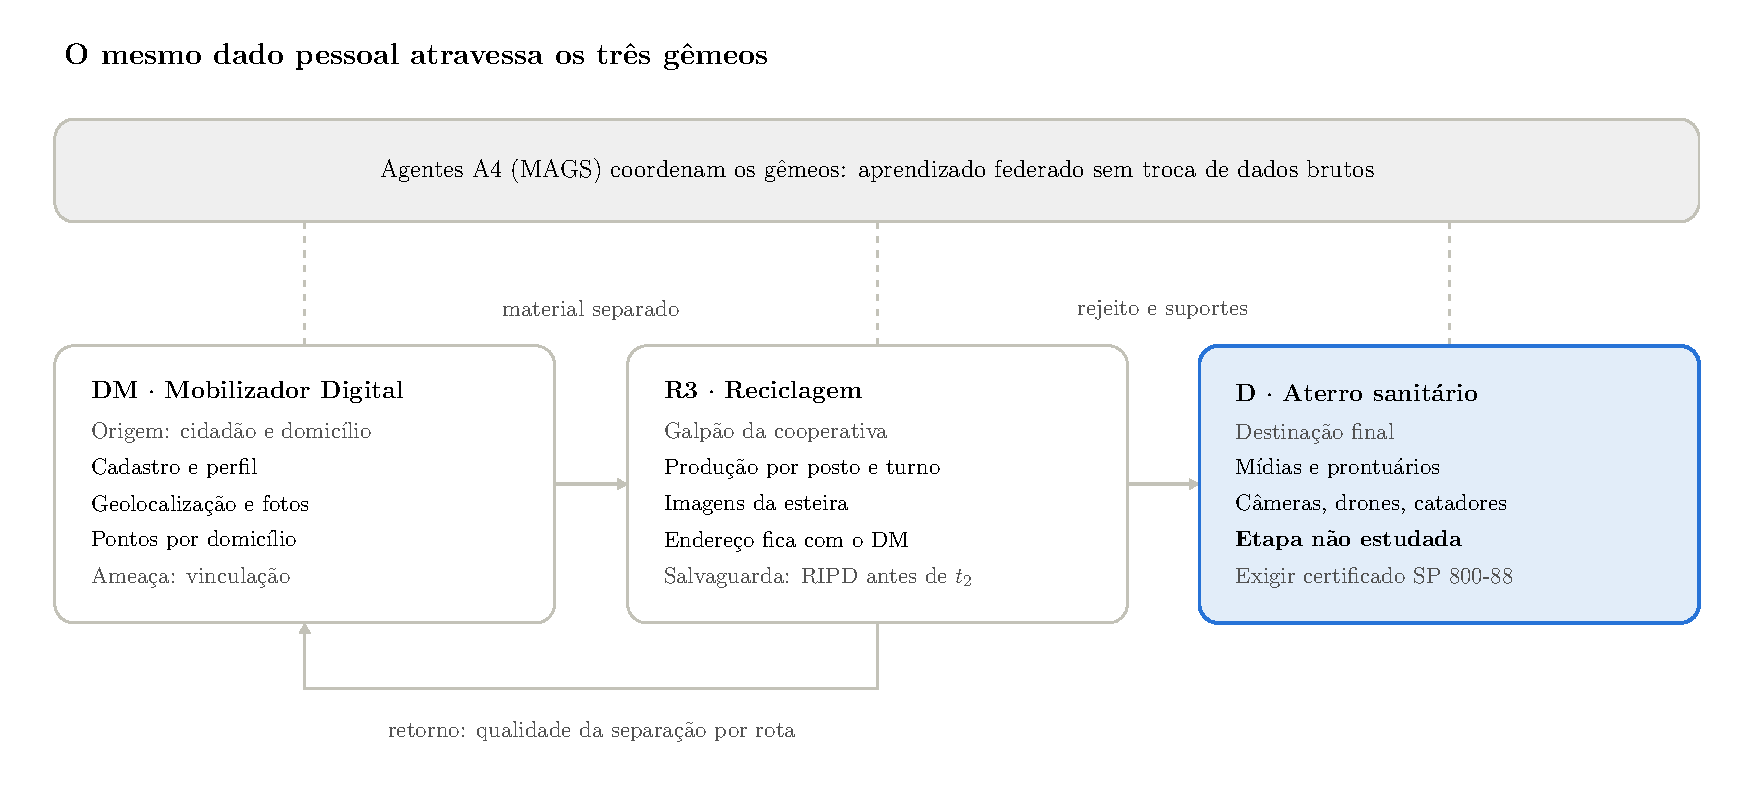
\includegraphics[width=\linewidth]{out/Figura_1_Percurso_Dado_Pessoal.pdf}
\fontetab{Elaborado pelo autor (2026), a partir dos três trabalhos base.}
\end{figure}

A Figura~\ref{fig:percurso} resume o percurso: o dado entra no DM, segue com o material até o R3, volta ao DM como qualidade por rota e chega ao aterro, a etapa que a literatura não estuda.

Dois pontos de cruzamento merecem atenção. O primeiro é o retorno da qualidade por rota do R3 ao DM: quanto menor a rota, mais próxima a informação fica do domicílio, e o trabalho do Aterro lembra que endereço, horário e peso por gerador são atributos que reidentificam. O segundo são os agentes A4, que no DM coordenam os gêmeos DM, R2, R3 e DS e no R3 coordenam cooperativas, SLU, compradores e outros gêmeos. O R3 já propõe a salvaguarda adequada --- aprendizado federado sem troca de dados brutos e acordos entre cooperativas ---, mas ela precisa valer para toda a rede, e não só para o lado da Reciclagem.

\subsection{Matriz consolidada}

A Tabela~\ref{tab:matriz} reúne, em uma única visão, o tratamento da privacidade em cada célula FSPC $\times$ segmento.

\begin{table}[!htbp]
\centering
\caption{Célula FSPC $\times$ segmento}
\label{tab:matriz}
\small
\begin{tabularx}{\linewidth}{>{\raggedright\arraybackslash}p{2.2cm} Y Y Y}
\hline
\textbf{Dimensão} & \textbf{DM \textperiodcentered{} Mobilizador} & \textbf{R3 \textperiodcentered{} Reciclagem} & \textbf{D \textperiodcentered{} Aterro}\\
\hline
Função & Perfil e pontuação por domicílio, implícitos & Monitoramento individual redesenhado para métricas por posto & Eliminação comprovada como função; certificado de sanitização\\
Estrutura & TW nomeada; \textit{blockchain} como registro imutável & Salvaguarda por agente (A1 a A4) & Densidade de sensores simulada contra reidentificação\\
Processo & Perfilamento na primeira etapa; risco alto sem etapa de tratamento & RIPD antes de \dsq{2}; imagens processadas no local & Ameaças LINDDUN por etapa; registro de riscos vivo\\
Contexto & LGPD declarada & Inventário com bases legais; princípios em decisões de projeto & Painel de conformidade; LGPD ausente da literatura\\
\hline
\end{tabularx}
\fontetab{Elaborado pelo autor (2026).}
\end{table}

Lida por colunas, a matriz mostra um gradiente de maturidade: o DM reconhece o risco, o R3 o converte em decisões de projeto e o Aterro o converte em função e em indicadores. Lida por linhas, mostra que cada segmento é mais forte em uma dimensão diferente, e que a descrição completa só aparece quando os três são lidos juntos.

\subsection{Arestas e faces: onde a privacidade se concentra}

O método do tetraedro permite uma leitura adicional. No R3, as arestas e faces que contêm o Contexto são as menos estudadas na literatura: FC tem 176 registros, SC 270 e a face FSC apenas 36. São também as que concentram a privacidade. Na aresta SC, a LGPD limita a estrutura de dados e define que os dados pertencem à cooperativa. Na face FSC, chamada pelo grupo de arquitetura institucional, estão a governança de dados pela cooperativa, os papéis, os consentimentos e os acordos de dados com SLU e compradores, apoiados nas capacidades MG e TW.

O Aterro chega ao mesmo lugar por outro caminho. A lacuna que ele mede é a Função de privacidade, mas o que falta é justamente a ligação entre Função e Contexto: a lei diz que o dado deve ser eliminado, mas a literatura não diz como verificar que um suporte descartado ficou ilegível. A convergência sugere que, nos gêmeos do SRS, a privacidade é uma propriedade das relações com o Contexto, e não de uma dimensão isolada, e que essas relações são as menos cobertas pela literatura.

\subsection{Implicações para a gestão de projetos}

Os três trabalhos ligam o gêmeo à gestão de projetos de modos diferentes. O DM alinha o projeto ao guia PMBOK por escopo, partes interessadas, ciclo de vida ágil, qualidade e riscos de TI --- com planos de segurança de dados --- e entrega de valor, medida pelo aumento da coleta seletiva e pela redução de custos logísticos. O R3 distribui o esforço na hierarquia de portfólios, programas, projetos e operações: a escala do dia e a alocação na esteira são operações; a implantação de cada configuração é projeto; a rede e os contratos são o programa P3RD; e a prioridade de investimento é o portfólio AEDR. O Aterro propõe que o gêmeo do sistema alimente o registro de riscos do gêmeo do projeto.

Para a privacidade, o Aterro identifica quatro dos sete domínios de desempenho do PMBOK 8 que precisam ser envolvidos, cada um ligado a uma função do NIST Privacy Framework:

\begin{table}[!htbp]
\centering
\caption{NIST Privacy Framework}
\label{tab:nist}
\small
\begin{tabularx}{\linewidth}{>{\raggedright\arraybackslash}p{3.2cm} >{\raggedright\arraybackslash}p{3cm} Y}
\hline
\textbf{Domínio do PMBOK 8} & \textbf{Função NIST} & \textbf{Papel na privacidade}\\
\hline
Governança & Govern-P & Define controlador e operador entre prefeitura, consórcio, coletora e aterro, e aprova o relatório de impacto\\
Partes interessadas & Communicate-P & Inclui titulares, catadores, comunidade do entorno e a ANPD\\
Recursos & Protect-P e Control-P & Trata sensores, nuvem e fornecedores como recursos que tratam dados, com cláusulas e controles\\
Risco & Identify-P & Cada ameaça LINDDUN vira um risco com gatilho medido pelo gêmeo e passa pelos seis processos de risco\\
\hline
\end{tabularx}
\fontetab{Elaborado pelo autor (2026).}
\end{table}

O mesmo trabalho propõe quatro critérios para tratar a Privacidade como domínio próprio --- objeto de risco próprio (o dano ao titular), métricas e unidades próprias, partes interessadas e obrigações próprias, e atividades em todo o ciclo de vida --- e um conjunto mínimo de indicadores, com metas ilustrativas a calibrar: 100\% dos fluxos com base legal e finalidade antes da operação; zero riscos ao titular significativos ou máximos sem resposta; $k \geq 10$ nos dados publicados por gerador; orçamento de privacidade diferencial definido e monitorado; 100\% dos lotes de mídia com sanitização verificada; e pedidos de titulares atendidos em até 15 dias.

A leitura conjunta mostra que esses critérios se aplicam aos três segmentos, e não só ao aterro. O objeto de risco próprio está nos domicílios do DM e nos catadores do R3; as métricas próprias se aplicam aos painéis públicos do DM e às métricas por posto do R3; as partes interessadas próprias incluem moradores, cooperados e a ANPD; e as atividades em todo o ciclo vão do perfilamento no DM à sanitização no aterro. O RIPD do R3, exigido antes de \dsq{2}, é um exemplo concreto de como esses critérios viram um ponto de decisão no ciclo do projeto.

% ------------------------------ 10 LIMITAÇÕES --------------------------------
\section{LIMITAÇÕES}

A consolidação herda as limitações dos três trabalhos base e acrescenta as suas.

\textbf{Limitações herdadas.} Os protocolos de busca são diferentes em base, período e cadeia, e por isso as contagens por dimensão não são comparáveis em valor absoluto. As contagens do R3 e do DM são indicadores lexicais: registram a presença do termo no tópico, e não a qualidade do tratamento da dimensão, como o próprio grupo da Reciclagem adverte. No Aterro, a triagem e a classificação por tema, categoria LINDDUN e dimensão FSPC foram feitas por expressões regulares sobre título, resumo e palavras-chave, o que super-representa temas de vocabulário amplo e pode perder estudos que tratam privacidade sem os termos da busca; a decisão final de elegibilidade depende da leitura do texto completo. O DM apoia-se em quatro artigos, e um deles (Banik et al., 2025) tem amostra de 20 participantes. O R3 descreve as cooperativas de forma genérica, com bases legais tratadas como hipóteses e metas de avanço ainda pendentes. Nenhum dos três gêmeos foi validado em campo.

\textbf{Limitações da consolidação.} A atribuição de trechos às células da matriz envolve julgamento, e trechos que tocam duas dimensões foram mantidos onde o trabalho original os colocou. Os pontos de privacidade que os trabalhos não explicitam foram derivados do texto pelas perguntas da seção 2.1, e estão sinalizados como leitura da consolidação. O artigo não acrescenta fontes externas, o que preserva a rastreabilidade, mas também significa que lacunas dos trabalhos base permanecem lacunas aqui. Por fim, a consolidação foi feita com apoio de inteligência artificial, nos termos declarados na seção 11.

% ------------------------------ 11 DECLARAÇÃO IA -----------------------------
\section{DECLARAÇÃO SOBRE O USO DE INTELIGÊNCIA ARTIFICIAL}

Esta consolidação foi produzida com apoio de inteligência artificial generativa. Os resultados de pesquisa pertencem aos grupos que os produziram; a IA foi usada para ler, organizar e redigir a síntese desses resultados, sob direção e revisão humanas.

\subsection{Ferramenta e período}

Foi usado o modelo de linguagem Claude, da Anthropic, em uma sessão do Claude (Cowork), em outubro de 2026. A sessão foi conduzida por um integrante do grupo Aterro, que forneceu os três trabalhos base e o Guia PMBOK 8 como arquivos e definiu, a cada etapa, o escopo e o formato das saídas.

\subsection{O que a IA fez}

\begin{enumerate}
\item \textbf{Leitura e extração.} Extraiu o texto dos três trabalhos e localizou os trechos que descrevem função, estrutura, processo e contexto, com seus dados numéricos e citações.
\item \textbf{Organização.} Atribuiu os trechos às células da matriz FSPC $\times$ segmento e comparou as células para identificar convergências, divergências e lacunas.
\item \textbf{Redação.} Redigiu o texto, as tabelas e a figura deste artigo, bem como uma análise preliminar e um pôster A1 com o mesmo conteúdo.
\item \textbf{Conferência pontual.} Em uma etapa anterior, conferiu no texto do PMBOK 8 as menções à privacidade descritas pelo trabalho do Aterro. Por decisão do condutor da sessão, a versão final se limita ao conteúdo dos três trabalhos base.
\end{enumerate}

\subsection{O que a IA não fez}

\begin{itemize}
\item Não executou buscas bibliográficas, não acessou as bases Web of Science ou Scopus e não gerou contagens, classificações ou dados novos. Todos os números citados vêm dos trabalhos base.
\item Não acrescentou fontes externas aos trabalhos base. As referências citadas são as que os próprios grupos usaram.
\item Não avaliou se, ou como, cada grupo usou ferramentas de IA na produção de seu trabalho. A autoria, os métodos e os resultados de cada trabalho base são responsabilidade do respectivo grupo, a quem cabe declarar o uso de IA em seu próprio texto.
\item Não é autora deste artigo. A IA não assume responsabilidade pelo conteúdo e não deve ser listada como autora.
\end{itemize}

\subsection{Riscos e salvaguardas}

Modelos de linguagem podem atribuir uma informação ao trabalho errado, simplificar um argumento a ponto de alterá-lo ou produzir afirmações plausíveis sem base no texto. Três salvaguardas foram adotadas: (1) a regra de usar apenas o conteúdo dos trabalhos base, que torna cada afirmação rastreável a um deles; (2) a separação explícita, nas seções 5 a 8, entre o que o trabalho afirma e o ponto de privacidade derivado pela consolidação; e (3) a revisão humana antes de qualquer submissão.

Recomenda-se que cada grupo confira as células referentes ao seu segmento, em especial números, citações e bases legais, antes que o texto seja apresentado ou submetido. Os trabalhos base não contêm dados pessoais além dos nomes dos autores, e nenhum dado pessoal de terceiros foi tratado na consolidação.

\subsection{Responsabilidade}

Cabe aos autores revisar o conteúdo gerado com apoio da IA antes da submissão; após essa revisão, respondem integralmente por ele. Esta declaração deve ser adaptada às políticas da disciplina, do programa e do veículo de publicação a que o artigo for submetido.

% ------------------------------ 12 CONCLUSÕES --------------------------------
\section{CONCLUSÕES E TRABALHOS FUTUROS}

Este artigo consolidou três trabalhos que descrevem gêmeos digitais de segmentos sucessivos do Sistema de Resíduos Sólidos do DF, organizando-os pelas quatro dimensões FSPC e lendo cada uma pelo domínio Privacidade. As respostas às três perguntas são estas.

\textbf{P1. O que cada segmento contribui.} O Mobilizador contribui com a origem do dado e com o anel bidirecional entre cidadão e gêmeo; a Reciclagem, com a descrição mais completa do gêmeo em FSPC, com a cadeia de configurações \dsq{k} e com salvaguardas de privacidade por agente e por dado; o Aterro, com o mapa de ameaças por etapa do ciclo, com a eliminação comprovada como função e com a ligação entre o gêmeo do sistema e o gêmeo do projeto.

\textbf{P2. Convergências e divergências.} Os três convergem no paradigma da referência, nas seis famílias de capacidades do DTC, no anel bidirecional e no marco PNRS e LGPD. Divergem na profundidade com que tratam a privacidade: o DM a reconhece como risco, o R3 a converte em decisões de projeto e o Aterro a converte em função e indicadores. Divergem também no que suas buscas dizem sobre o Contexto: pouco estudado na literatura de reciclagem e de mobilização, muito estudado na de privacidade, mas sem chegar a direitos, instituições e à LGPD.

\textbf{P3. O que só a leitura conjunta revela.} O mesmo dado pessoal atravessa os três gêmeos, e seus pontos de cruzamento --- o retorno da qualidade por rota e os agentes de rede A4 --- não pertencem a nenhum segmento isoladamente. A privacidade se concentra nas relações com o Contexto (as arestas FC e SC e a face FSC), que são as menos estudadas. E a etapa em que o dado deveria deixar de existir, a destinação final, é a única sem estudo.

Cinco frentes de trabalho decorrem dessas conclusões, todas apontadas ou sugeridas pelos trabalhos base:

\begin{enumerate}
\item \textbf{Registro único de tratamentos.} Unificar o inventário de dados do R3 com os fluxos do DM e do Aterro em um registro por gêmeo, com as bases legais validadas pelo encarregado de dados, como o R3 prevê para a próxima fase.
\item \textbf{Acordos de dados entre gêmeos.} Estender a salvaguarda do A4 do R3 --- aprendizado federado sem troca de dados brutos --- a toda a rede de gêmeos do SRS, e definir a granularidade mínima do retorno de qualidade por rota.
\item \textbf{Protocolo de sanitização.} Desenvolver, como propõe o Aterro, um protocolo de verificação de sanitização (NIST SP 800-88) com certificado rastreável até o aterro.
\item \textbf{FMEA de privacidade dinâmica.} Transformar a avaliação pontual de risco em registro vivo, atualizado por dados de operação dos três gêmeos.
\item \textbf{Validação em campo.} Validar as descrições com ao menos uma cooperativa e com o SLU, como prevê o R3, e realizar a prova de conceito de gêmeo de projeto em um aterro piloto, como prevê o Aterro.
\end{enumerate}

Lidos separadamente, os três trabalhos descrevem três gêmeos. Lidos juntos, descrevem uma cadeia, e a privacidade só pode ser garantida se for gerida como propriedade dessa cadeia.

% ------------------------------ REFERÊNCIAS ----------------------------------
\begin{center}
\textbf{REFERÊNCIAS}
\end{center}

\begingroup
\SingleSpacing
\setlength{\parindent}{0pt}
\setlength{\parskip}{12pt}
\raggedright

ALCARAZ, C.; LOPEZ, J. Digital twin: a comprehensive survey of security threats. \textbf{IEEE Communications Surveys \& Tutorials}, v. 24, n. 3, 2022.

BANIK, Bijoy et al. A Mobile Platform for Smart Recycling and Eco-Friendly Sustainable Environment. \textbf{Journal of Social Innovation and Knowledge}, v. 2, p. 150-175, 2025.

BRASIL. Decreto nº 10.936, de 12 de janeiro de 2022. Regulamenta a Lei nº 12.305/2010. Brasília, DF, 2022.

BRASIL. Decreto nº 11.413, de 13 de fevereiro de 2023. Institui o Certificado de Crédito de Reciclagem de Logística Reversa e outros certificados. Brasília, DF, 2023.

BRASIL. Lei nº 12.305, de 2 de agosto de 2010. Institui a Política Nacional de Resíduos Sólidos. Brasília, DF, 2010.

BRASIL. Lei nº 13.709, de 14 de agosto de 2018. Lei Geral de Proteção de Dados Pessoais (LGPD). Brasília, DF, 2018.

BRIGHENTE, A.; CONTI, M.; DI RENZONE, G.; PERUZZI, G.; POZZEBON, A. Security and privacy of smart waste management systems: a cyber-physical system perspective. \textbf{IEEE Internet of Things Journal}, 2024. DOI: 10.1109/JIOT.2023.3322532.

BROOKS, S.; GARCIA, M.; LEFKOVITZ, N.; LIGHTMAN, S.; NADEAU, E. \textbf{An introduction to privacy engineering and risk management in federal systems}. NISTIR 8062. Gaithersburg: NIST, 2017.

CHEN, H.; TUREL, O.; YUAN, Y. E-waste information security protection motivation: the role of optimism bias. \textbf{Information Technology \& People}, 2022. DOI: 10.1108/ITP-09-2019-0458.

DENG, M.; WUYTS, K.; SCANDARIATO, R.; PRENEEL, B.; JOOSEN, W. A privacy threat analysis framework: supporting the elicitation and fulfillment of privacy requirements. \textbf{Requirements Engineering}, v. 16, n. 1, p. 3--32, 2011.

DIGITAL TWIN CONSORTIUM. \textbf{Digital Twin Capabilities Periodic Table (v. 1.2) e AI Agent Capabilities Periodic Table (v. 1.0)}. Boston: DTC, 2025.

FONSECA-MEDRANO, M. C. et al. Characterization of solid wastes as a tool to implement waste management strategies in a university campus. \textbf{International Journal of Sustainability in Higher Education}, v. 21, n. 7, 2020.

FUKAMI, A.; REGAZZONI, F.; GERADTS, Z. Data sanitization on eMMCs. In: \textbf{ASIA AND SOUTH PACIFIC DESIGN AUTOMATION CONFERENCE (ASP-DAC)}, 2023. DOI: 10.1145/3566097.3568349.

GARFINKEL, S. L.; SHELAT, A. Remembrance of data passed: a study of disk sanitization practices. \textbf{IEEE Security \& Privacy}, v. 1, n. 1, p. 17--27, 2003.

GHARAJEDAGHI, J. \textbf{Systems thinking: managing chaos and complexity}. 3. ed. Burlington: Morgan Kaufmann, 2011.

GIEL, R.; DĄBROWSKA, A. Digital twin concept for manual waste sorting management. \textbf{Environment Protection Engineering}, v. 51, n. 1, p. 65--74, 2025. DOI: 10.37190/epe250104.

GRIEVES, M.; VICKERS, J. Digital twin: mitigating unpredictable, undesirable emergent behavior in complex systems. In: KAHLEN, F.-J.; FLUMERFELT, S.; ALVES, A. (ed.). \textbf{Transdisciplinary perspectives on complex systems}. Cham: Springer, 2017.

JOSHI, S.; SHARMA, M.; BARVE, A. Implementation challenges of blockchain technology in closed-loop supply chain: a WEEE management perspective in developing countries. \textbf{Supply Chain Forum: An International Journal}, 2023. DOI: 10.1080/16258312.2022.2135972.

KRITZINGER, W.; KARNER, M.; TRAAR, G.; HENJES, J.; SIHN, W. Digital twin in manufacturing: a categorical literature review and classification. \textbf{IFAC-PapersOnLine}, v. 51, n. 11, p. 1016--1022, 2018. DOI: 10.1016/j.ifacol.2018.08.474.

LEAL, A. E. F. et al. Applications of digital technologies for overcoming challenges in municipal solid waste reverse logistics: a systematic literature review. \textbf{Engenharia Sanitária e Ambiental}, v. 29, 2024.

LI, X. Personal information security risk assessment for e-waste recycling based on Fuzzy-GRA-TOPSIS and FMEA. \textbf{IEEE Transactions on Engineering Management}, 2024. DOI: 10.1109/TEM.2024.3395649.

NISSENBAUM, H. Privacy as contextual integrity. \textbf{Washington Law Review}, v. 79, n. 1, p. 119--157, 2004.

NIST. \textbf{NIST Privacy Framework: a tool for improving privacy through enterprise risk management, version 1.0}. Gaithersburg: NIST, 2020.

NIST. \textbf{SP 800-88 Rev. 1: guidelines for media sanitization}. Gaithersburg: NIST, 2014.

NOLASCO, Elaine et al. Characterization of solid wastes as a tool to implement waste management strategies in a university campus. \textbf{International Journal of Sustainability in Higher Education}, v. 22, n. 4, p. 805-824, 2021.

OLAWADE, D. B. et al. Smart waste management: a paradigm shift enabled by artificial intelligence. \textbf{Waste Management Bulletin}, 2024. DOI: 10.1016/j.wmb.2024.05.001.

OLIVEIRA, G. P.; REIS, M. V. O.; ARCANJO, S. A.; SILVA, W. A. \textbf{Projeto prático: componente de sistema de resíduos sólidos urbanos -- Mobilizador Digital 1}. Brasília: UnB/PPCA, Gestão de Projetos de TI, 2026.

PMI -- PROJECT MANAGEMENT INSTITUTE. \textbf{A guide to the project management body of knowledge (PMBOK guide)}. 8. ed. Newtown Square: PMI, 2025.

PRATA, J.; SIMÕES, C. L.; SIMÕES, R. Improvements to municipal solid waste collection systems using real-time monitoring. \textbf{Sustainability}, v. 17, n. 4, 1405, 2025.

ROCHA, L.; SILVA, E.; GARCIA, H.; FERREIRA, L. \textbf{Privacidade no descarte de resíduos sólidos: atualização SIPA da revisão sobre aterros sanitários sob a ótica FSPC (v2)}. Brasília: UnB/PPCA, Gestão de Projetos de TI, 2026.

ROCHER, L.; HENDRICKX, J. M.; DE MONTJOYE, Y.-A. Estimating the success of re-identifications in incomplete datasets using generative models. \textbf{Nature Communications}, v. 10, art. 3069, 2019.

SOUSA, F. A.; CORREIA, E. B. G.; SILVA, R. I. D.; PAPA, C. E. S. \textbf{Gestão do gêmeo digital de reciclagem em cooperativas sob a ótica da privacidade (SIPA)}. Entrega P2A. Brasília: UnB/PPCA, Gestão de Projetos de TI, 2026.

TAO, F. et al. Digital twin in industry. \textbf{IEEE Transactions on Industrial Informatics}, v. 15, n. 4, p. 2405--2415, 2018.

WANG, H.; ZHENG, L.; XUE, Q.; LI, X. Research on medical waste supervision model and implementation method based on blockchain. \textbf{Security and Communication Networks}, 2022. DOI: 10.1155/2022/5630960.

\endgroup

\end{document}
